% Prelim, Chapter 2
% by Rachel Slaybaugh

\chapter{Upscattering and Energy Decomposition}
\label{sec:Chp2}
The first piece that was added to Denovo to accelerate the code was the multigroup Krylov solver. The second two methods rely on the energy decomposition and improved convergence added by this solver, so its functionality is essential to all subsequent work. The multigroup Krylov solver works very well and is a key element in accomplishing the goals of this work. 

First, why the existing parallel decomposition in Denovo is insufficient for solving challenging problems is explained. Next, the background section discusses scattering and some solver basics, including an overview of Krylov subspace methods and why they are of interest for solving the transport equation. The next section focuses on existing methods used to solve the fixed source transport equation and relevant past work. Finally, a description of the new method and associated results are presented.

\section{Denovo and Parallelism}
To be able to solve the very large problems of interest on machines the size of Jaguar, codes that have good scaling properties are required. Recall that Denovo can be parallelized in space and angle. This is done with the Koch-Baker-Alcouffe (KBA)\cite{Baker1998} parallel sweep algorithm on a Cartesian grid. The KBA algorithm governs Denovo's parallel behavior, including how many cores it can efficiently use. To see why parallelization in energy is needed, the KBA algorithm is explained and some illustrative Denovo calculations are presented

Angular parallelization is done by algorithmically ``stacking'' the calculation directions (ordinates) into a ``pipe'' and following more than one at one time. The transport sweeps begin with the first direction in the first quadrant and spatially move through the geometry along that ordinate in a hyper-plane fashion. Denovo uses a pipelining approach in direction such that the next angle set in an octant is started as soon as the current sweep reaches the opposite end of the geometry. The quadrants are ordered such that the next quadrant begins at the earliest possible time \cite{Evans2009d}. 

The spatial decomposition is done by assigning groups of spatial cells to different cores. A given problem will contain $(I, J, K)$ total global \emph{cells}. These are decomposed in $x$ and $y$ across $P_{I}$ cores in the $x$-direction and $P_{J}$ cores in the $y$-direction for a total of $P_{I} \times P_{J}$ cores. Each core gets a \emph{domain} that is made up of $(I_{b}, J_{b}, K)$ cells. Here $I_{b} = I/P_{I}$ and $J_{b} = J/P_{J}$. Each domain is algorithmically split into $B_{K}$ computational blocks in the $z$-direction (but not split in memory, all $K$ cells in the $z$-direction are on all cores). This creates \emph{computational blocks} of size $(I_{b}, J_{b}, K_{b})$, where $K_{b} = K/B_{K}$. The computational blocks are used in the angular pipelining process. Specifying the number of cores dictates $P_{I}$ and $P_{J}$, while the user is free to select $B_{K}$. See Figure \ref{fig:BlockDecomp} for an example of a decomposition.

\begin{figure}[!ht]	
  \begin{center}
    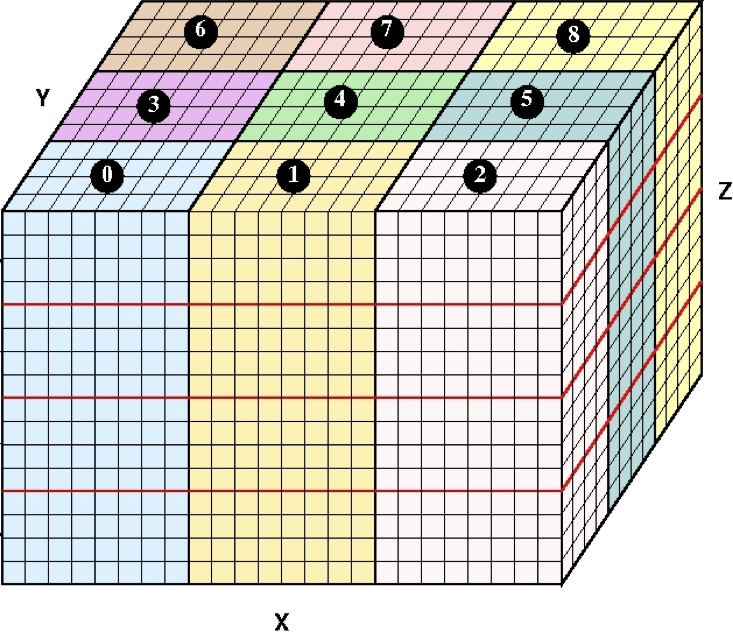
\includegraphics [width=0.6\textwidth, height=0.4\textheight ] {BlockDecompCropped}
  \end{center}
  \caption{Decomposition of 3-D mesh for KBA. In this example, the grid is decomposed on nine processors. The red lines indicated computational blocks in the $z$-direction. Each processor has $I_{b} \times J_{b} \times K$ cells, and each computational block has size $I_{b} \times J_{b} \times K_{b}$.}
  \label{fig:BlockDecomp}
\end{figure}

The decomposition parameters can be used to express the theoretical efficiency of the algorithm, which is the ratio of useful computations to total computations \cite{Evans2009d}, \cite{Baker1998}:
%
\begin{equation}
  \epsilon_{max} = \frac{2MB_{K}}{2MB_{K} + P_{I} + P_{J} - 2} \:, 
  \label{eq:efficiency}
\end{equation}
%
where $M$ is the number of directions in an octant. Note that for a set $M$, $P_{I}$, and $P_{J}$, the theoretical efficiency will be much higher when there is a larger $B_{k}$, meaning more computational blocks. Having more computational blocks creates blocks that are smaller, so work can be passed to subsequent blocks more rapidly and thus more work should be able to be done at once. See \cite{Baker1998} for more details about the KBA algorithm.

The quality of parallelization can be measured in several ways. Strong scaling measures how the time to solution varies with the number of cores for a fixed problem size. Weak scaling measures how the time to solution varies with the addition of more cores when the problem size per core is fixed \cite{Bush2010}. Another factor is the total number of cores that can be used efficiently. 

A weak scaling study was performed by Evans et.\ al.\ on the Jaguar machine using a full-facility PWR model. The base-case time was generated using 4,096 cores with 103,716,288 unknowns, or $\sim$25,300 unknowns/core. When 40,000 cores and 1,046,879,390 unknowns ($\sim$26,200 unknowns/core or about a 3\% increase in problem size/core) were used, there was a 43\% increase in time to solution. The time increase for perfect weak scaling would have been about 3\%. The significant increase in time can be attributed to load-balancing latencies associated with KBA \cite{Evans2009d}. Adding parallelization over energy might improve the weak scaling properties of denovo by making up for some of the latencies that come from KBA.

The author conducted a strong scaling study on the Jaguar machine that investigated the effect of $B_{K}$ on efficiency. A variant of the Kobayashi benchmark problem 1 \cite{Kobayashi2000}, which can be seen in Figure~\ref{fig:Kob1}, was used where the total cross sections were changed as indicated in Table~\ref{tab:Kob1xsecs}. The scattering cross sections were simply set to 0.5 $\times \Macro$ in both the original and modified case. The calculation was done with $S_{16}/P_{0}$, step characteristic spatial differencing, and a 0.25 cm spatial resolution, giving a 400 $\times$ 400 $\times$ 400 mesh.  The number of cores was varied between 12 and 3,600. 

\begin{figure}[!ht]	
  \begin{center}
    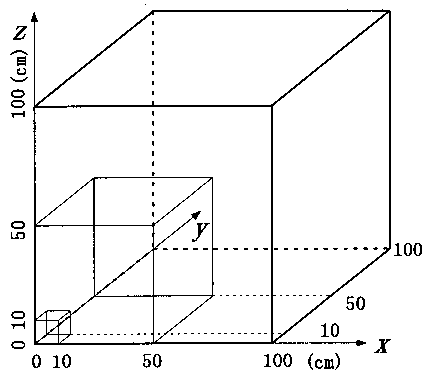
\includegraphics [width=0.4\textwidth, height=0.3\textheight ] {Kobayashi1} \\
    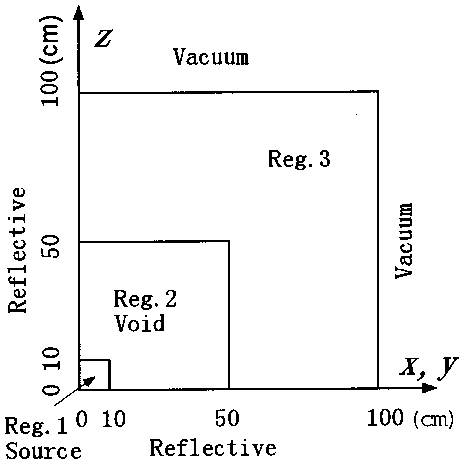
\includegraphics [width=0.4\textwidth, height=0.3\textheight ] {Kobayashi1Front}
  \end{center}
  \caption{Two Views of the Kobayashi Benchmark Problem 1}
  \label{fig:Kob1}
\end{figure}

\begin{table}[h]
  \caption{Cross Sections and Sources for Kobayashi Benchmark Problem 1}
  \centering
  \begin{tabular}{|c|c|c|c|}
    \hline
    Region & S & Original $\Macro$ & Modified $\Macro$ \\
    (\#) & ($n$ cm$^{-3}$s$^{-1}$) & (cm$^{-1}$) & (cm$^{-1}$) \\
    \hline
    1 & 1 & 0.1 & 1 \\
    2 & 0 & 10$^{-4}$ & 10$^{-3}$ \\
    3 & 0 & 0.1 & 1 \\
    \hline
  \end{tabular}
  \label{tab:Kob1xsecs}
\end{table}

The author did one set of calculations using $B_{K}$ = 40, or relatively many blocks, and one set using $B_{K}$ = 5, or relatively few blocks. Recall from Equation \eqref{eq:efficiency} that more computational blocks should give higher efficiency. The theoretical and actual results are plotted in Figure~\ref{fig:JagBlockStudy} as computational efficiency as a function of the number of cores used. The actual efficiency is $\frac{N_{ref}t_{ref}}{Nt}$. Here $N_{ref}$ and $t_{ref}$ are the reference number of cores and solve time, respectively, and $N$ and $t$ are for the calculation in question.  The theoretical efficiency was calculated using Equation \eqref{eq:efficiency}.

\begin{figure}[!h]
  \begin{center}
    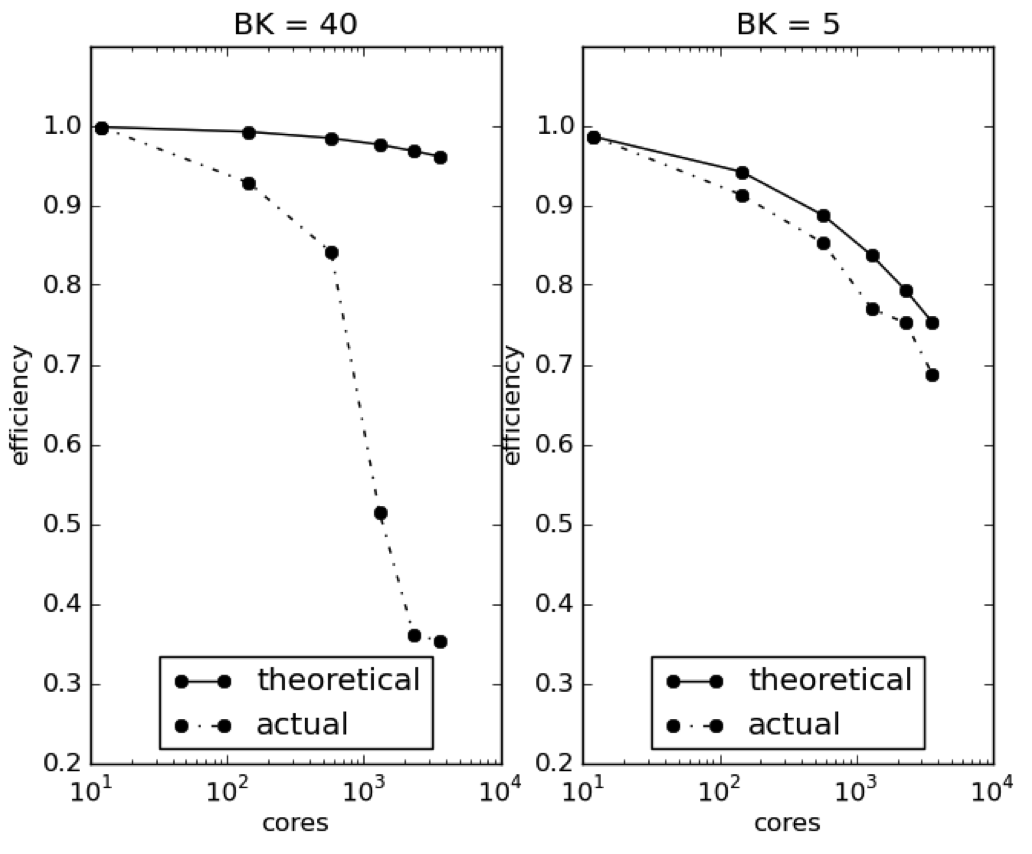
\includegraphics [width=.9\textwidth, height=0.5\textheight ] {JagBlockStudy}
  \end{center}
  \caption{Efficiency as a Function of Number of Cores for the Modified Kobayashi 1 Problem}
  \label{fig:JagBlockStudy}
\end{figure}

A few important conclusions can be drawn from the curves in Figure~\ref{fig:JagBlockStudy}. One is that the increase in simultaneous work that should come from using smaller computational blocks is overwhelmed by communication latency in practice. When $B_{K}$ = 40 the theoretical efficiency remains high as the number of cores increases, but the measured efficiency becomes quite low: for 3,600 cores $\epsilon_{max}$ = 0.96 and $\epsilon$ = 0.35. It is expected that more blocks would be better, but when the number of cells/block becomes too small the cores spend more time waiting to pass data than doing floating point operations (flops). 

Another relevant finding is that the theoretical and actual efficiencies match when there is a minimum block size. When larger computational spaces are used (smaller $B_{K}$) communication does not become a dominant factor. This restricts the extent of spatial decomposition by limiting the number of blocks used for a given spatial mesh. For a 500M cell problem, the limitation is 15,000 - 20,000 cores. 

As a result of all of this, a problem can only be decomposed so far for a given mesh before communication latency begins to dominate solution time and using more cores will be of little benefit. This is caused by the KBA algorithm. In order to take advantage of more cores for a given problem size, another area of phase space must be parallelized: energy, the remaining unparallelized dimension. 

%--------------------------------------------------------------------------------
%--------------------------------------------------------------------------------
\section{Background}
To understand the new method and why it enhances Denovo's performance, some background information is required. This section contains an explanation of scattering, an overview of relevant basic solvers, and information about how we handle scattering in the transport equation. The remainder of this chapter will primarily focus on the solution of $\ve{A}x = b$, where $\ve{A}$ is $n \times n$  and the exact form of $\ve{A}$ and $b$ will be specified in subsequent sections.

%--------------------------------------------------------------------------------
\subsection{Scattering}
One of the important contributions of this work is the implementation of a new way to handle upscattering in transport calculations. When neutrons scatter, several outcomes with regard to energy are possible. One outcome is that neutrons can stay within their energy group, which is called within-group scattering and is described by the $[\ve{S}]_{gg}$ portion of the scattering matrix. Neutrons can also move into a lower energy group, or downscatter, which is given by $[\ve{S}]_{gg'}$ where $g > g'$. In some cases neutrons can gain energy and upscatter, described by $[\ve{S}]_{gg'}$ where $g < g'$. 

Material cross sections can be highly energy dependent and therefore high-resolution data in certain energy ranges may be needed to accurately capture the physics of the system. Upscattering is often important in problems where detailed information about low-energy, or thermal, neutrons is needed. In light-water reactors, thermal neutrons cause the bulk of the fission so these are systems that often need cross sections with upscattering terms.  

As mentioned in Chapter \ref{sec:Chp1}, the transport problem is broken into outer iterations and inner iterations. The inner iterations correspond to within-group the equations. Each inner iteration converges the flux for just one group by solving a fixed source problem for that group. The fixed source contains the appropriate combination of inscattering from other groups, an external source, and a source from fission.  The outer iterations are over the entire set of energy groups - all of Equations \eqref{eq:group-equations}. If a problem does not have upscattering, the equations can be quickly solved using one outer iteration. 

%--------------------------------------------------------------------------------
\subsection{Solver Basics}
There are two categories of methods for solving $\ve{A}x = b$, direct and iterative. Direct methods solve the problem by inverting $\ve{A}$ and setting $x = \ve{A}^{-1}b$. If $\ve{A}$ is invertible this can be done explicitly. $\ve{A}$ is often not invertible, so most direct methods are based on factoring the coefficient matrix $\ve{A}$ into matrices that are easy to invert. The problem is then solved in pieces where each factored matrix is inverted to get the final solution. An example where this is done is LU factorization. These methods are often robust and require a predictable amount of time and storage resources. However, direct methods scale poorly with problem size, becoming increasingly expensive as problems grow large \cite{Benzi2002}.

Iterative methods compute a sequence of increasingly accurate approximations to the solution. They generally require less storage and take fewer operations than direct methods, though they may not be as reliable. Iterative methods are highly advantageous for large problems because direct methods become intractable for systems of the size of those of interest here. For this reason the nuclear energy industry tends to use iterative methods for transport calculations \cite{Birkhoff1984}, \cite{Benzi2002}. 

\subsubsection{Richardson Iteration}
The simplest iteration scheme used by the nuclear community is source iteration (SI), also known as Richardson iteration. SI is applied to the within-group space-angle iterations. Some other method is needed to conduct outer iterations over energy. Richardson iteration can be thought of as a two-part process for the neutron transport equation, where $\bar{Q}$ includes all sources and $k$ is the inner iteration index:
%
\begin{align}
  \ve{L}\psi_g^{k+1} &= \ve{MS} \phi_g^k + \bar{Q} \:,   \label{eq:SIpsi} \\
  \phi_g^{k+1} &= \ve{D}\psi_g^{k+1} \:.
  \label{eq:SIphi}
\end{align}
%
The spectral radius determines the speed of convergence and is $c = \frac{\Macro_s}{\Macro}$. For problems that are dominated by scattering, SI will converge very slowly \cite{Evans2009d}. While this is the simplest iterative method used, there are much more sophisticated methods available. 

\subsubsection{Gauss Seidel}
Gauss Seidel (GS) is known as the method of successive displacements \cite{LeVeque2007}. It is commonly used as the outer iteration method over energy and can be written as follows where $j$ is the outer iteration index:
%
\begin{equation}
  \ve{L} [\psi]_{g}^{j+1} = [\ve{M}] [\ve{S}]_{gg}[\phi]_{g}^{j+1} +   [\ve{M}]\bigl(\sum_{g'=1}^{g-1} [\ve{S}]_{gg'}[\phi]_{g'}^{j+1} + \sum_{g'=g+1}^{G} [\ve{S}]_{gg'}[\phi]_{g'}^{j} + [q_{e}]_{g} \bigr) \label{eq:GaussSeidel} \:. 
\end{equation}
%
The GS method is implicit and contains terms on the right hand side at both the new and old iteration levels. Once the space-angle iterations for each upscattering group are completed for one outer iteration, the right hand side is recalculated and the within-group calculations are repeated. This goes on until the entire system converges \cite{Evans2009d}. 

Gauss Seidel is unconditionally stable, but may converge very slowly. The convergence of GS is governed by its spectral radius, $\rho$ \cite{LeVeque2007}. The spectral radius of Gauss Seidel has been found for various materials by solving the eigenvalue problem $(\ve{T} - \ve{S}_{D})^{-1}\ve{S}_{U} \xi = \rho \xi$, where $\ve{T}$ is the matrix of total cross sections and $\xi$ is the eigenvector. This eigenvalue problem comes from Fourier analysis. The spectral radii for some materials of practical interest determined using cross sections with 41 thermal upscattering groups are: graphite = 0.9984, heavy water = 0.9998, and iron = 0.6120 \cite{Adams2002}. Problems containing graphite or heavy water would converge very slowly if GS were used.   

\subsubsection{Krylov methods}
Krylov methods\footnote{For a detailed discussion of Krylov methods and how they work see Appendix \ref{sec:AppendixB}} are a powerful class of subspace methods that can be ideal for solving various types of linear and eigenvalue problems. A Krylov method solves $\ve{A}x = b$ by building a solution from a Krylov subspace generated by an iteration vector $v_{1}$. At iteration $k$, the subspace is:
%
\begin{equation}
  \mathcal{K}_{k}(\ve{A},v_{1}) \equiv span\{v_{1}, \ve{A}v_{1}, \ve{A}^{2}v_{1}, ..., \ve{A}^{k-1}v_{1}\} \:.
  \label{eq:Krylov-subspace}
\end{equation}
%
The choice of $v_{1}$ varies, but $v_{1} = b$ is common. When the problem is presented as $\ve{A}z = r_{0}$ where $r_{0} \equiv b - \ve{A}x_{0}$ and the solution is $x_{k} = x_{0} + z$, then $v_{1} $ is often chosen to be $r_{0}$. Note that $x_{0}$ is the initial guess and $x_{k}$ is the solution approximation at step $k$  \cite{Ipsen1998}.

The dimension of a Krylov space is bounded by $n$ because Krylov methods will give the exact solution after $n$ iterations if roundoff error in neglected. Interestingly, this technically makes Krylov methods a hybrid of direct and iterative methods because an exact answer can be obtained in a set number of steps. Krylov subspace methods are nevertheless generally classified as iterative methods \cite{Birkhoff1984}.

Krylov methods are particularly useful in a few pertinent cases. One is when $\ve{A}$ is very large because fewer operations are required than traditional inversion methods like Gaussian elimination. Another is when $\ve{A}$ is not explicitly formed because Krylov methods only need the action of $\ve{A}$. Finally, Krylov methods are ideal when $\ve{A}$ is sparse because the number of operations are low for each matrix-vector multiplication. For deterministic transport codes, $\ve{A}$ is typically quite large, fairly sparse, and only its action is needed. The action of $\ve{A}$ is implemented through the transport sweeps \cite{Lewis1993}, \cite{Ipsen1998}.  

In the last few decades Krylov methods have been used widely to solve problems with appropriate properties for several reasons. Krylov methods are robust; the existence and uniqueness of the solution can be established; typically far fewer than $n$ iterations are needed when they are used as iterative solvers; they can be preconditioned to significantly reduce time to solution; only matrix-vector products are required; explicit construction of intermediate residuals is not needed; and they have been found to be highly efficient in practice \cite{Ipsen1998}, \cite{Knoll2004}. 

There are, however, a few drawbacks. In some cases Krylov methods can be very slow to converge, causing large subspaces to be generated and thus becoming prohibitively expensive in terms of storage size and cost of computation. Some methods can be restarted after $m$ steps\footnote{For information about restarted Krylov methods see Appendix \ref{sec:AppendixB}} to alleviate this problem, keeping the maximum subspace size below $\mathcal{K}_{m+1}$.  The relatively inexpensive restart techniques can reduce the storage requirements and computational costs associated with a slow-converging problem such that they are tractable. Preconditioners can also help by reducing the number of iterations needed. Development of appropriate preconditioners is an active area of research \cite{Warsa2004a}, \cite{Ipsen1998}, \cite{Knoll2004}. 

In the 1970s interest in Krylov methods in the wider computational community began to increase after it was demonstrated that these methods can converge quickly. At first Krylov methods were restricted to problems where $\ve{A}$ is symmetric positive definite (SPD). These are methods such as conjugate gradient (CG), MINRES, SYMMLQ, and others. Then, Krylov methods for non-symmetric matrices became a focus, including the Generalized Minimum Residual (GMRES) and BiConjugate Gradient Stabilized (BiCGSTAB) methods \cite{Barrett1994}, \cite{Benzi2002}. The transport problem has characteristics that make it well suited for solution with Krylov methods, and these methods are used in several novel ways throughout this work.

%--------------------------------------------------------------------------------
\subsection{Current Scattering Solution Methods}
All three of the methods just discussed are used in many transport codes, including Denovo. The inner iterations are done with either SI or a Krylov method and the outer iterations are done with Gauss Seidel. In this chapter the energy block consists of the upscattering block. The operator notation developed in Chapter~\ref{sec:Chp1} is used throughout the balance of this work. The fixed source problem will be presented here, but the discussion can be easily extended to eigenvalue calculations by using the fission source for each group in place of the external source. 

A simple five group example matrix will be used for reference throughout this section. The matrix illustrates the structure of $\ve{S}$  when groups 1 and 2 have only downscattering and the upscatter block is defined over the range [$g_{1}$ = 3, $g_{2}$ = 5]:
%
\begin{equation}
  \mathbf{S}  =     \begin{pmatrix}
      [\ve{S}]_{11} &0 & 0 & 0 & 0 \\
      [\ve{S}]_{21} & [\ve{S}]_{22} & 0 & 0 & 0 \\
      [\ve{S}]_{31} & [\ve{S}]_{32} & [\ve{S}]_{33} & [\ve{S}]_{34} & [\ve{S}]_{35} \\
      [\ve{S}]_{41} & [\ve{S}]_{42} & [\ve{S}]_{43} & [\ve{S}]_{44} & [\ve{S}]_{45} \\
      [\ve{S}]_{51} & [\ve{S}]_{52} & [\ve{S}]_{53} & [\ve{S}]_{54} & [\ve{S}]_{55}
    \end{pmatrix} \:.
    \label{eq:exmp-matrix}
\end{equation}

\subsubsection{Downscattering}
Groups that only contain downscattering can be solved using forward substitution. The within-group transport equations are the same as in Equation \eqref{eq:GaussSeidel}, but the upscattering term goes away. The equation is combined with Equation \eqref{eq:SIphi} and rearranged to eliminate $[\psi]_{g}$ such that the unknown quantity is $[\phi]_{g}$. 

Each group equation is solved sequentially starting with group $1$, so all group moments on the right hand side have already converged for the $j+1$ outer iterate. To help clarify notation, the moments being iterated upon will be designated $\phi^{*}$, the moments which are known at the $j+1$ iterate will be $\phi^{new}$ and those from $j$ will be $\phi^{old}$. Together this looks like:
\begin{align}
  &[\phi]_{g}^{*} =  \ve{DL^{-1}}[\ve{M}][\ve{S}]_{gg}[\phi]_{g}^{*} +  \ve{DL^{-1}}[\ve{M}] \bigl(  \sum_{g'=1}^{g-1} [\ve{S}]_{gg'}[\phi]_{g'}^{new} + [q_{e}]_{g} \bigr) \label{eq:within-unarranged} \:;  \\
  %
  &\underbrace{\bigl( \ve{I} - \ve{DL^{-1}}[\ve{M}][\ve{S}]_{gg} \bigr)}_{\tilde{\ve{A}}}[\phi]_{g}^{*} = \underbrace{\ve{DL^{-1}}  [\ve{M}] \bigl(  \sum_{g'=1}^{g-1} [\ve{S}]_{gg'}[\phi]_{g'}^{new} + [q_{e}]_{g} \bigr) }_{\tilde{b}} \label{eq:within-krylov} \:. 
\end{align}
%
For example matrix \eqref{eq:exmp-matrix}, the first and second groups would be solved using this strategy. That means forward substitution would be used to solve this part of the scattering matrix:
%
\begin{equation}
  \mathbf{S_{down}} = \begin{pmatrix}
      [\ve{S}]_{11} &0 & 0 & 0 & 0 \\
      [\ve{S}]_{21} & [\ve{S}]_{22} & 0 & 0 & 0 \\  
      \end{pmatrix} \:.
          \label{eq:down-matrix}
\end{equation}
%
For group 2, Equation~\eqref{eq:within-krylov} would be:
%
\begin{equation}
  \bigl( \ve{I} - \ve{DL^{-1}}[\ve{M}][\ve{S}]_{22} \bigr)[\phi]_{2}^{*} = \ve{DL^{-1}}[\ve{M}] \bigl( [\ve{S}]_{21}[\phi]_{1}^{new}  + [q_{e}]_{1} \bigr) \:.
\end{equation}

Once the equations have been arranged in this way, a within-group solver is used to find the $j+1$ value for $[\phi]_{g}$. This iterative method could be source iteration, a Krylov method, or some other choice. When using a Krylov solver, the first step is always to calculate $\tilde{b}$. 

In Denovo, Aztec \cite{Heroux2007} provides the linear within-group solver. The Aztec solver is given an operator that implements the action of $\tilde{\ve{A}}$, the right hand side $\tilde{b}$, and an iteration/solution vector $v$. The action of $\tilde{\ve{A}}$ is implemented by doing the following for a group $g$:
\begin{enumerate}
  \item matrix-vector multiply: $y_{g} = [\ve{M}][\ve{S}]_{gg} v_{g}$,
  \item sweep: $z_{g} = \ve{DL}^{-1} y_{g}$,
  \item return: $v_{g} \leftarrow v_{g} - z_{g}$.
\end{enumerate}
In this implementation the Aztec solver iterates on $v_{g}$, which represents $[\phi]_{g}$, until it is converged for that group. Once the updated moments are returned, the next group is iterated upon. 

An iterative solver is used for even these simple forward substitution calculations because $\tilde{\ve{A}}$ is never explicitly formed and thus Equation \eqref{eq:within-krylov} cannot be solved directly. Only one outer iteration is required in fixed source problems when there is no upscattering because once each group is converged it is not changed by lower energy groups. 

Another way to look at this is that the right hand side of the equation is not changed by subsequent iterations, so solving $[\tilde{\ve{A}}]_{g} [\phi]_{g} = [\tilde{b}]_{g}$ will give the same answer both before and after all subsequent downscattering moments, $[\phi]_{g'}, g' \ne g$, are determined. Because this procedure is so straightforward, there is no motivation to parallelize it in energy for fixed source problems.

\subsubsection{Upscattering}
When upscattering is present, the lower energy groups do influence the higher energy groups so multiple outer iterations are needed. The within-group equations for groups $[g_{1}, g_{2}]$ now contain contributions from both higher and lower energy groups. 

The Gauss-Seidel (GS) method is commonly used to handle the upscattering block and, using the same notation as the downscattering section, can be written as follows:
%
\begin{equation}
\underbrace{\bigl( \ve{I} - \ve{DL^{-1}}[\ve{M}][\ve{S}]_{gg} \bigr)}_{\tilde{\ve{A}}} [\phi]^{*}_{g} = \underbrace{\ve{DL^{-1}}[\ve{M}] \bigl( \sum_{g'=1}^{g-1}[\ve{S}]_{gg'}[\phi]^{new}_{g'} + \sum_{g'=g+1}^{g2} [\ve{S}]_{gg'}[\phi]^{old}_{g'}  + [q_{e}]_{g} \bigr)}_{\tilde{b}}  \:.
 \label{eq:up-GS}
\end{equation}
%
Because lower energy groups that haven't been solved yet contribute neutrons to higher energy groups that have already been solved, the upscatter block becomes its own iteration loop. The solution procedure is exactly the same as with downscattering only, except that once the $[\phi]_{g_{1}}$ to $[\phi]_{g_{2}}$ moments are converged $\tilde{b}$ is recalculated and the outer iterations over the upscatter block are repeated. Most deterministic transport codes use GS for upscattering. In GS, all upscattering groups are coupled together so parallelization over energy is not possible \cite{Evans2009d}. 

%-----------------------------------------------------------
%-----------------------------------------------------------
\section{Past Work}
Now that the basics of inner and outer iterations have been described, past solution methods can be understood. 

\subsection{Inner Iterations}
Source iteration was historically the inner iteration method of choice. SI is still often used, but now it is typically accelerated to improve convergence. Unfortunately, even accelerated SI is not always fast or robust enough for new calculations of interest. The slow convergence of SI is part of what motivated interest in Krylov methods. 

In 1977 CG, which requires $\ve{A}$ to be symmetric positive definite (SPD), was used in solving the transport equation for the first time \cite{Lewis1977}. $\ve{A}$ is only SPD for the discretized transport equation when a symmetric quadrature set is used for the \Sn approximation and the scattering is isotropic. Otherwise, the matrix is non-symmetric. GMRES, which works for non-symmetric systems, was applied in a transport problem with anisotropic scattering for the first time in 1991 \cite{Adams2002}. It was not until Krylov methods for non-symmetric matrices were developed, restart methods became well known, and computer architecture could accommodate the storage required by Krylov subspaces needed in transport problems that the nuclear community began more widely using Krylov methods. 

With a few exceptions, Krylov methods have only been applied to the inner iterations for neutron transport. In some cases Krylov methods have been used as stand-alone iterative schemes to perform the within-group solves. In other cases they have been used as one part of the inner iteration process. For example, diffusion or transport synthetic acceleration (D/TSA) is often chosen to precondition SI as the inner iteration solver, where CG is used to solve the D/TSA portion of the calculation \cite{Gupta2004}. Krylov methods have also been applied to the diffusion equation when a few groups have been used \cite{Suetomi1988}, \cite{Verdu1999}.

Krylov methods have so far been largely restricted to inner iterations or few-group diffusion problems primarily because of hardware limitations and momentum of existing code structure. A Krylov subspace of size 30 can use a lot of memory when $v$ holds many variables. Until very recently, computers were not large enough to handle subspace iteration methods for a 3-D, anisotropic transport problem with many energy groups.  

Further, the inner-outer iteration structure has been successfully used in computational neutronics for quite some time, and it can take substantial effort to modify the fundamental solution processes in large codes. Often there is a time lag between when new methods are developed and when they find wide-spread incorporation, which adds to the delay in implementing new methods in existing codes.

\subsection{Outer Iterations}
When upscattering is present, Gauss Seidel is almost universally used as the outer iteration solver. As noted above, GS can converge very slowly for some systems containing materials like heavy water, which are of interest to the nuclear community. Such slow convergence is part of the motivation for this work, which develops a method to replace GS for the upscatter block. 

There is one case where a Krylov method was used in a fixed source problem for something besides within-group solves. In 2004 Warsa et.\ al.\ used restarted flexible GMRES as an intermediate-level iteration over upscatter groups (what this chapter calls the outer iterations). In one upscattering case they used a Krylov solver for within-group iterations, FGMRES(m) over the upscatter block, and an implicitly restarted Arnoldi method for the eigenvalue outer iteration. They compared this to using block GS for the upscatter intermediate-level iteration. They found that using a Krylov solver rather than block Gauss Seidel for upscatter was faster. This is the only work found by the author that used a Krylov method for upscattering \cite{Warsa2004a}. 

Choosing to use an intermediate-level Krylov solver while still doing inner iterations with a Krylov solver is a bit of a strange choice. As far as the author can tell, this choice was motivated by the desire to minimize changes to the code. By keeping the traditional inner-outer iteration method and adding a Krylov layer in between, very little code modification was needed. 

The methods that have been used in the past dictate an inner-outer iteration structure and limit parallelization to space and angle. The author was unable to find transport codes that have been parallelized in energy nor ones that deal with upscattering in a way different from what has been explained above. 

%-----------------------------------------------------
%----------------------------------------------------- 
\section{Multigroup Krylov Solver}
The ``Denovo and Parallelism'' section demonstrated that Denovo is limited in the number of cores it can use effectively. In addition to enhanced parallelism, there is also a need for faster solution algorithms for all parts of the code so Denovo can be used to solve very large systems. To address these issues, a new solver was implemented that applies a Krylov method to an entire block of energy groups rather than to only one group at a time. This replaces the inner-outer iteration structure with just one level of iteration because all groups can be converged simultaneously. 

\subsection{Method}
The first goal of this project is to decouple energy groups so that the energy portion of phase space can be parallelized. This goal can be achieved in a straightforward way for an upscattering block by solving the entire block as one entity with a Krylov method rather than solving one group at a time. 

In the new method, the downscatter groups are treated the same way as before. For the example case, $[\phi]_{1}$ and $[\phi]_{2}$ are solved in the downscattering only calculations and are known by the time the upscatter block is reached. The portion of the scattering matrix shown in Equation \eqref{eq:up-source-matrix}, operates on these moments. 
%
 \begin{equation}
  \mathbf{S_{up\_source}}  =     \begin{pmatrix}
      [\ve{S}]_{31} & [\ve{S}]_{32}  \\
      [\ve{S}]_{41} & [\ve{S}]_{42}  \\
      [\ve{S}]_{51} & [\ve{S}]_{52} 
    \end{pmatrix} \:,
    \label{eq:up-source-matrix} 
 \end{equation}
%
The remainder of the scattering matrix, shown in Equation \eqref{eq:up-matrix}, operates on $[\phi]_{3-5}$. The idea behind the new solver is to treat $[\phi]_{3-5}$ as one vector to be solved at one time, rather than three vectors to be solved in series. 
%
 \begin{equation}
  \mathbf{S_{up\_block}}  =     \begin{pmatrix}
      [\ve{S}]_{33} & [\ve{S}]_{34} & [\ve{S}]_{35} \\
      [\ve{S}]_{43} & [\ve{S}]_{44} & [\ve{S}]_{45} \\
      [\ve{S}]_{53} & [\ve{S}]_{54} & [\ve{S}]_{55}
    \end{pmatrix} \:.
    \label{eq:up-matrix}
\end{equation}

Instead of $\tilde{G} = g_{2 }- g_{1}$ separate within-group upscattering equations, the new method has \emph{one} block upscattering equation. To do this, Equation \eqref{eq:up-GS} is modified to apply to a block instead of a series of groups. The entire upscatter block, or matrix \eqref{eq:up-matrix}, moves to the left because it acts on the upscattering-block-vector being iterated upon ($[\phi]_{3-5} = \phi^{*}$). The upscatter source, $\ve{S}_{\text{up\_source}}$ of matrix \eqref{eq:up-source-matrix} remains on the right because it is only acting on the downscattering groups that have been solved at the current iteration level ($[\phi]_{1-2} = \phi^{new}$). The form of the new strategy is shown in Equation \eqref{eq:up-krylov} and looks very much like Equation \eqref{eq:up-GS}.
%
\begin{equation}
 \underbrace{ \bigl( \ve{I} - \ve{DL^{-1}}\ve{M}\ve{S}_{\text{up\_block}} \bigr)}_{\tilde{\ve{A}}} \phi^{*} = \underbrace{ \ve{DL^{-1}}\ve{M} \bigl( \ve{S}_{\text{up\_source}}\phi^{new} + q_{e} \bigr)}_{\tilde{\ve{b}}}  \label{eq:up-krylov} \\
\end{equation}

Applying the Krylov solver to this system is very similar to what was done before, but now the action of $\ve{\tilde{A}}$, or the matrix-vector multiply, is applied to the entire block at once instead of just one group:
%
\begin{enumerate}
  \item matrix-vector multiply: $y = \ve{M}\ve{S}_{\text{up\_block}} v$,
  \item sweep: $z = \ve{DL}^{-1} y$,
  \item return: $v \leftarrow v - z$.
\end{enumerate}
%
All that has happened to allow for solving the entire block at once is the redefinition of the iteration vector. The scattering terms are still coupled together through physical cross sections, but the way they contribute to one another is addressed all at one time through Krylov iteration rather than serially through Gauss Seidel iteration. 

This new formulation allows for parallelization of the upscatter groups in energy. The matrix vector multiply can be done at the same time for all upscattering groups for each iteration. To see how this works, refer to Figure \ref{fig:KrylovMultiply}. Each color can do its part of the matrix vector multiply at the same time as the other colors. After the separate multiplies, there is a global reduction so that every color has the updated s, or the same brown box. The rest of the application of A is straightforward and doesn't require any inter-color communication \cite{Evans2010}.
%
\begin{figure}[!h]
  \begin{center}
    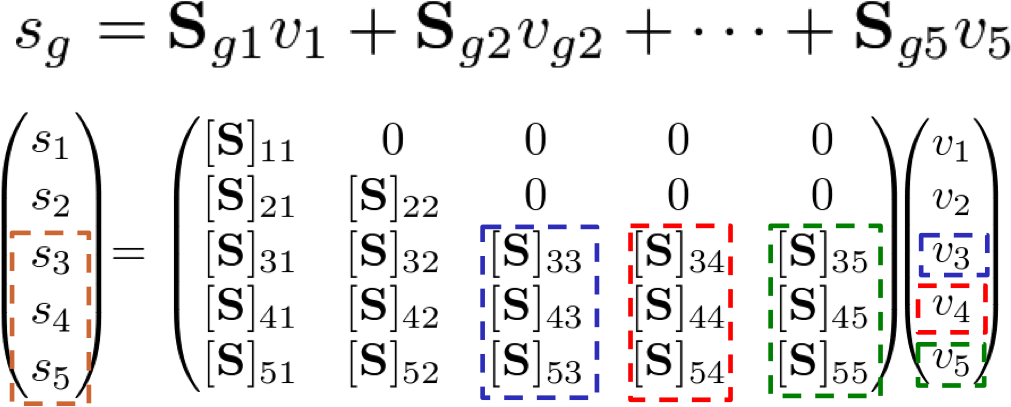
\includegraphics [width=.6\textwidth, height=0.2\textheight ] {KrylovGroupMultiply}
  \end{center}
  \caption{Parallel Implementation of Upscattering Matrix-Vector Multiply}
  \label{fig:KrylovMultiply}
\end{figure}

To accomplish the parallelization, the problem is broken up into \emph{energy sets}. There can be between $1$ and $\tilde{G}$ sets; the groups are distributed evenly among sets. Each energy set gets the entire spatial mesh, so the spatial decomposition does not change. Because the full mesh is on each set, KBA  can be used just like before and it does not have to cross any spatial boundaries or scale to where it becomes inefficient. A picture of the decomposition can be seen in Figure \ref{fig:EnergyDecomp}.
%
\begin{figure}[!h]
  \begin{center}
    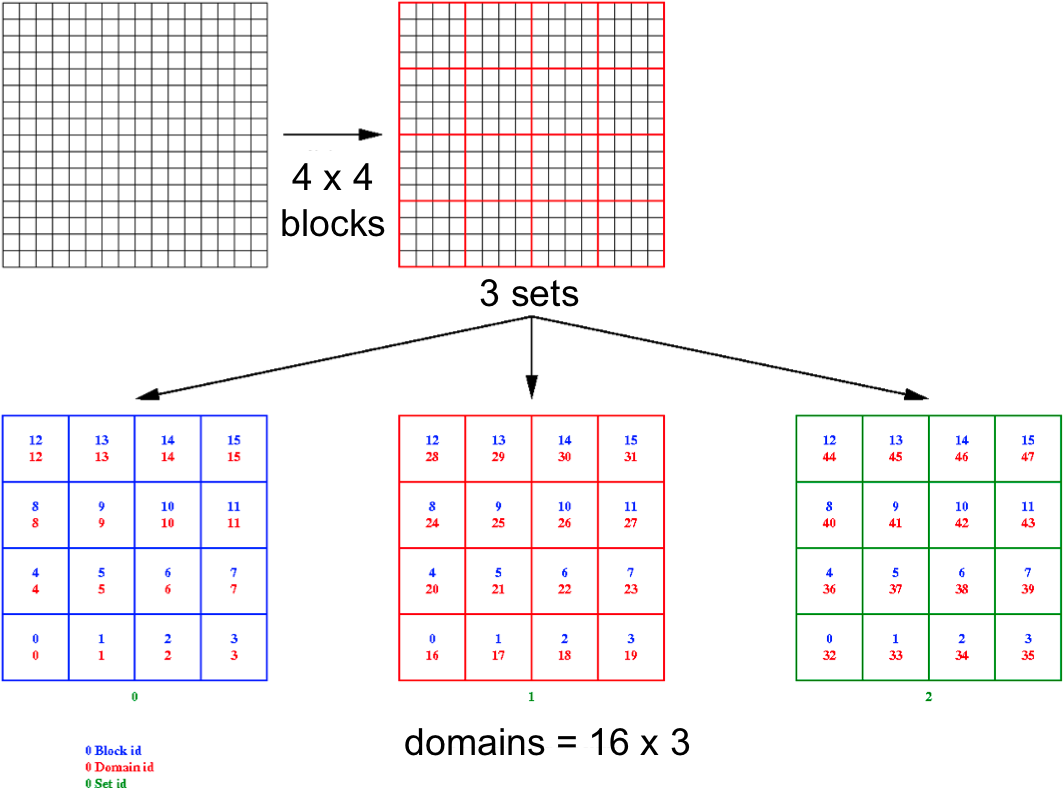
\includegraphics [width=.8\textwidth, height=0.45\textheight ] {EnergySets}
  \end{center}
  \caption{Energy Set Decomposition Added to Denovo \cite{Evans2011}}
  \label{fig:EnergyDecomp}
\end{figure}

It was demonstrated in Section 1 that KBA becomes latency dominated when block size becomes small, limiting the number of cores that can be used for a given problem. With energy decomposition, more cores can be used without requiring KBA to scale further because scaling can be done across energy instead of space-angle. 

The number of cores is set by the number of domains. Previously, the number of domains was equal to the number of spatial blocks. Now it is the number of energy sets $\times$ the number of spatial blocks. With the addition of sets Denovo can use hundreds of thousands of cores. For example, with 10,000 spatial blocks (which KBA can handle) and 10 energy sets, Denovo can use 100,000 cores \cite{Evans2011}, \cite{Evans2010}. KBA would not be able to efficiently use 100,000 spatial blocks. This dramatically increases the scalability of Denovo.

Before this work, no one had decoupled the transport equation in energy nor used one iteration level instead of two. We can now do this because we have machines large enough to store Krylov subspaces made from multiple group-sized iteration vectors, and these computers are large enough to warrant parallelization in energy . 

%--------------------------------------------------------------------------------
\subsection{Results}
The new method, which will be referred to as multigroup (MG) Krylov or block Krylov, has been implemented in Denovo. Two test problems were used to investigate the benefits of the new method. One was simply a small toy problem and the other was a full scale reactor calculation. Energy decomposition was investigated from the standpoint of both strong and weak scaling. The problems were also run without energy decomposition, i.e.\ using one energy set, to compare using Krylov instead of GS for the upscatter groups. First MG Krylov and GS are compared, then strong scaling studies are shown, and finally weak scaling is discussed.

\subsubsection{Gauss Seidel vs. Block Krylov}
The first problem used to compare GS to MG Krylov for multigroup upscattering was the toy problem. This is a cube of half of iron and half graphite discretized with a 50 $\times$ 50 $\times$ 50 orthogonal mesh and decomposed into two spatial domains to use two cores. It is a 27-group problem with 13 upscattering groups and vacuum boundary conditions. An isotropic source is assigned everywhere to the first three energy groups, and the problem used $P_0$, and $S_4$. The iron plus graphite material composition was chosen for several reasons. Both materials are commonly found in nuclear reactors, graphite is highly scattering and creates a system with a large spectral radius for GS, and the cross sections were available with multiple upscattering groups.

The calculation took $3.51 \times 10^{3}$ seconds using MG Krylov, and the upscattering block converged in 43 GMRES iterations. With GS, the calculation took $2.87 \times 10^{4}$ seconds, or 718\% longer. This case converged in 44 Gauss Seidel iterations, each of which took about 124 GMRES inner iterations, or $\sim$5455 GMRES iterations all together. Note that the Krylov iterations in MG Krylov needed a subspace with a length dimension of 13 energy groups while the Krylov iterations in GS had a length of 1 energy group. This means the cost of the GMRES applications is not the same between solvers. Despite this, GS was very clearly more costly.

Next a more realistic problem, a full pressurized water reactor (PWR) core, was tested by Evans on the Jaguar machine. This PWR has 289 17 $\times$ 17 assemblies (157 fuel, 132 reflector) and vacuum boundary conditions. There are low, medium, and high enrichment fuel pins. A 2 $\times$ 2 spatial discretization per homogenized fuel pin was used giving 233,858,800 cells. $S_{12}$ was selected as the angular discretization. Two energy groups were used for this test to keep the total problem size small. To get a sense of the problem size, there were 78,576,556,800 unknowns.

It should be noted that Jaguar requires decompositions to be done in a certain way, which determines the number of domains that can be used. For example, exactly doubling domain size is typically not possible so the closest available approximation is chosen instead.

\begin{table}[!h]
\caption{MG Krylov - GS Comparison for the Full PWR}
\begin{center}
\begin{tabular}{l c c c c}
\hline
Solvers & Blocks & Sets & Domains & Solver Time (min) \\[0.5ex]
\hline
PI + TTG GS & 17,424 & 1 & 17,242 & 11.00 \\
PI + MG Krylov & 10,200 & 2 & 20,400 & 3.03 \\
\hline
\end{tabular}
\end{center}
\label{table:MGkrylovPWR}
\end{table}
%
Table~\ref{table:MGkrylovPWR} shows the results for the full PWR problem. The goal was to compare MG Krylov and GS using the same number of domains, which required a different spatial decomposition. Power Iteration (described in Chapter~\ref{sec:Chp3}) was used for the eigenvalue solver in both cases; GS again used GMRES for the inner iterations. For this problem GS was accelerated with a two-grid preconditioner (TTG; details are given in Section~\ref{sec:TTG}). While GS had 15.5\% fewer domains than MG Krylov, it took 263\% longer. Clearly the MG Krylov method was much faster than GS for this problem, even when GS was preconditioned and MG Krylov was not. 

In both test cases the new Krylov multigroup solver significantly outperformed Gauss Seidel. The Krylov method took much less time and many fewer iterations, even when Gauss Seidel was accelerated. This demonstrates that the new multigroup solver provides substantial convergence improvement, which will help solve large and challenging problems. 

\subsubsection{Strong Scaling}
The two test problems were also used to examine strong scaling with energy sets. The iron graphite calculations were not as much a scaling study as a qualitative indication of whether the energy set decomposition works. The as expanded to a 100 $\times$ 100 $\times$ 100 mesh and decomposed into four spatial blocks to make it large enough to warrant using multisets. It should be noted that it is not expected that this problem will scale particularly well because dividing 13 groups into energy sets will result in load imbalance. There is no way to evenly divide the number of sets among cores, meaning at least one processor always has one more group than the others. The cores with fewer groups must wait for the cores with more groups. The more sets used, the larger the number of cores waiting.

The number of energy sets was varied from 1 to 13. The test problems were run on the small Orthanc cluster at ORNL. The results can be seen in Figure~\ref{fig:FeGraphiteStudy}. The downscattering groups were solved with forward substitution as before, and the upscattering was solved with the Krylov multigroup solver. The upscattering groups converged in 104 GMRES iterations.

\begin{figure}[!h]
  \begin{center}
    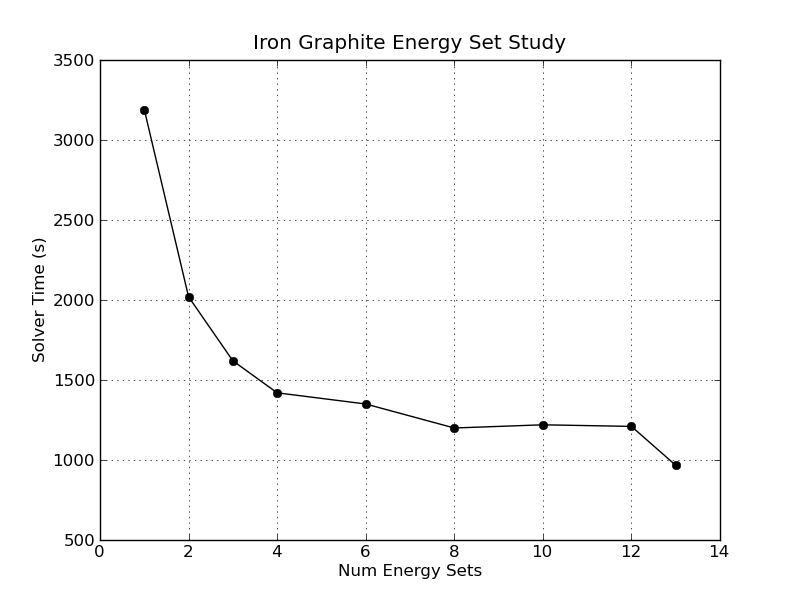
\includegraphics [width=.85\textwidth, height=0.5\textheight ] {FeGraphiteEnergyStudy}
  \end{center}
  \caption{Solver Time vs. Energy Decomposition for the Iron-Graphite Toy Problem}
  \label{fig:FeGraphiteStudy}
\end{figure}
%
The results indicate that decomposing over energy does reduce solution time. Going from one to two energy sets, or doubling the number of cores, reduces the time to solution by 37\%. Using four energy sets reduces the solve time by 56\%. Using more than a few energy sets for this problem  does not give significant payback in solve time. This is not too surprising as it was not expected that this problem would scale well because of load balancing issues. The point, however, is that some speedup was seen and the decomposition and solver work correctly.

A 44 energy group cross section set was used with the PWR to study strong scaling in a more quantitative way than the toy problem. This many energy groups gave 1,728,684,249,900 degrees of freedom. Three decomposition combinations were used, detailed in Table~\ref{table:StrongCasesPWR}. Each case used power iteration and the MG Krylov solver. Because of the decomposition restrictions, 9,024 spatial domains was the closest available approximation to 10,200, and 5,040 domains was closest to half.
%
\begin{table}[!h]
\caption{Strong Scaling for the Full PWR Problem Decomposition}
\begin{center}
\begin{tabular}{l c c c c}
\hline
Case & Blocks & Sets & Domains & Solver Time (min) \\[0.5ex]
\hline
I   & 10,200 & 11 & 112,200 & 49.61 \\
II  & 5,040   & 22 & 110,880 & 53.61 \\
III & 9,024   & 22 & 198,528 & 34.99 \\
\hline
\end{tabular}
\end{center}
\label{table:StrongCasesPWR}
\end{table}

Case III was compared to Case I to examine the effect of doubling the number of energy groups with the spatial decomposition fixed. Case III was compared to Case II to examine the effect of doubling the spatial decomposition with the energy sets fixed. If perfect, i.e.\ linear, scaling were obtained, the solve time would be $(\frac{\text{base\_domains}}{\text{used\_domains}}) \times \text{base\_time}$. The efficiency can be defined as the $\frac{\text{t\_perfect}}{\text{t\_actual}}$. 

\begin{table}[!h]
\caption{Full PWR Case III Comparison}
\begin{center}
\begin{tabular}{l c c c c}
\hline
Compare To & Perfect & Actual & Efficiency \\[0.5ex]
\hline
I  (energy)  & 28.04 & 34.99 & 0.80 \\
II  (space) & 29.94 & 34.99 & 0.86\\
\hline
\end{tabular}
\end{center}
\label{table:StrongPWRresults}
\end{table}
%
The comparison results are shown in Table~\ref{table:StrongPWRresults}. The timing results, plotted with a linear scaling line for reference, are shown in Figure~\ref{fig:PWRstrongScaling}. Both of the results are quite good. Doubling the energy sets resulted in an efficiency of 80\%. This is slightly less than the efficiency of 86\% that came from doubling the spatial decomposition. Neither case differs drastically from linear scaling. 
%
\begin{figure}[!h]
  \begin{center}
    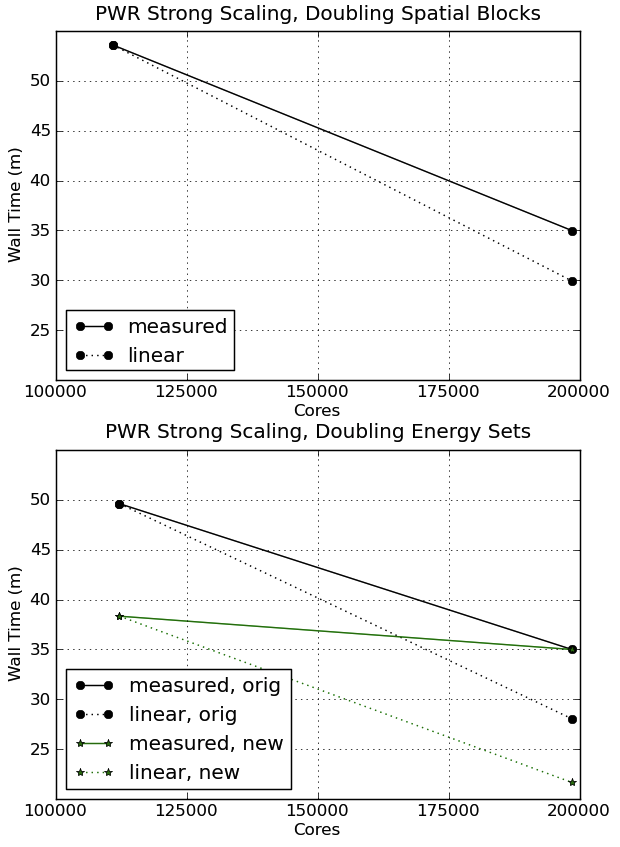
\includegraphics [width=.6\textwidth, height=.75\textheight ] {PWRstrongScaling}
  \end{center}
  \caption{Strong Scaling Study for the Full PWR Calculation with 44 Groups}
  \label{fig:PWRstrongScaling}
\end{figure}

Some general communication optimization was added to Denovo after these initial results were obtained and Cases I and III were re-run. The optimization greatly improved the Case I results, reducing the solve time from 53.61 minutes to 38.33 minutes. Unfortunately, there was very little difference in run time for Case III and the scaling efficiency reduced to 62\%. %A plot of the new results and comparison to linear scaling can be seen in Figure~\ref{fig:NewStrongScaling}. 
%%
%\begin{figure}[!h]
%  \begin{center}
%    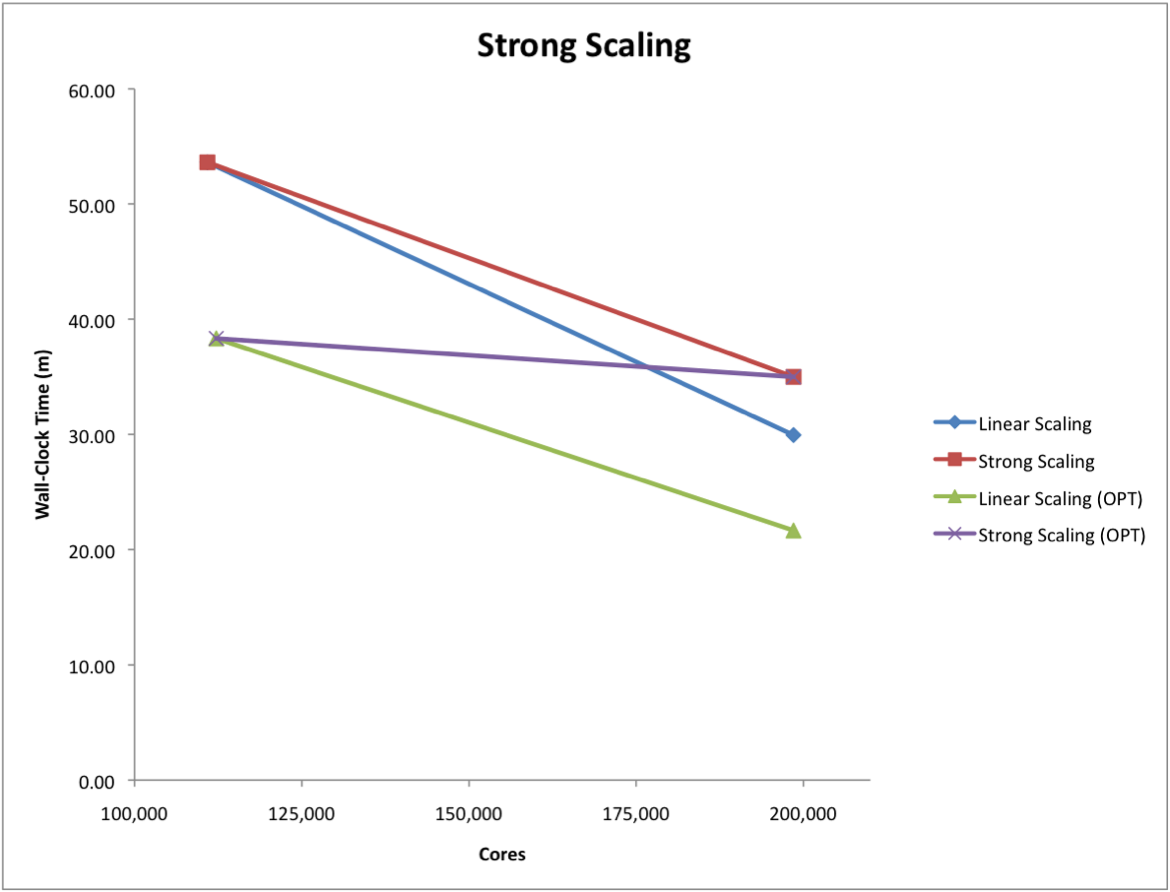
\includegraphics [width=.8\textwidth, height=.51\textheight ] {NewStrongScalingPWR}
%  \end{center}
%  \caption{Strong Scaling Study With Communication Optimization for the Full PWR Calculation with 44 Groups}
%  \label{fig:NewStrongScaling}
%\end{figure}

A variety of reasons have been identified for why the 200,000-core case did not improve as much as the 100,000-core case. Many of these are beyond the scope of this work: it is likely that the problem is not large enough to demonstrate strong scaling well; the block decomposition was not optimal; there were communication collisions on the torus across the full machine that significantly slowed down communication. Pertinent to this work, however, is that the multiset communication was not optimal. After each matrix-vector multiply a global reduction and scatter were done. In that process every space-energy domain communicated its updated flux to every other space-energy domain, which can be slow. 

This communication pattern has since been improved to a global reduction followed by a local scatter. That means when each space-energy domain communicates its updated flux after the multiply it only communicates it to the cores with the same spatial domains, not to all cores. This improvement has been implemented, but the calculations have not yet been repeated. With this improvement alone, better strong scaling behavior would likely result. 

Despite the reduction in strong scaling performance, one of the most important results from these calculations is the number of cores that were used successfully. Denovo was able to use 100,00 to 200,000 cores when it was previously limited to about 20,000. It also solved a problem with over 1.7 trillion degrees of freedom in 40 minutes. These results demonstrate that the multigroup Krylov solver allows for the use of leadership-class machines.

\subsubsection{Weak Scaling}
Finally, the full PWR problem was used for a weak scaling study. The two-group, 17,424-block, GS calculation from the previous subsection (PI + TTG GS in Table~\ref{table:MGkrylovPWR}) was compared to the 44-group, 11-set, 10,200-block, MG Krylov calculation with the optimized communication strategy. 

Recall that there were 78,576,556,800 unknowns when using 2 groups with 1 set on 17,424 cores, and 1,728,684,249,900 unknowns when using 44 groups with 11 sets on 112,200 cores. With weak scaling the problem size/core is typically kept constant. In this case the problem size/core could not be held constant, so an adjustment factor was included. The number of energy groups were used to weight the problem size/core and that was used to get an adjusted solve time of 11.21 minutes for the MG Krylov calculation: $[(\frac{44}{2})(\frac{17,424}{112,200})]^{-1}\times38.33$ = 11.21. 

Efficiency for weak scaling is calculated by taking the ratio of the MG Krylov adjusted time to the reference time, or 11.21 over 11.00, giving an efficiency of 1.019. A plot of the weak scaling is shown in Figure~\ref{fig:PWRweakScaling}. Note that perfect weak scaling would maintain an efficiency of 1, thus the weak scaling observed here was very good. 
%
\begin{figure}[!h]
  \begin{center}
    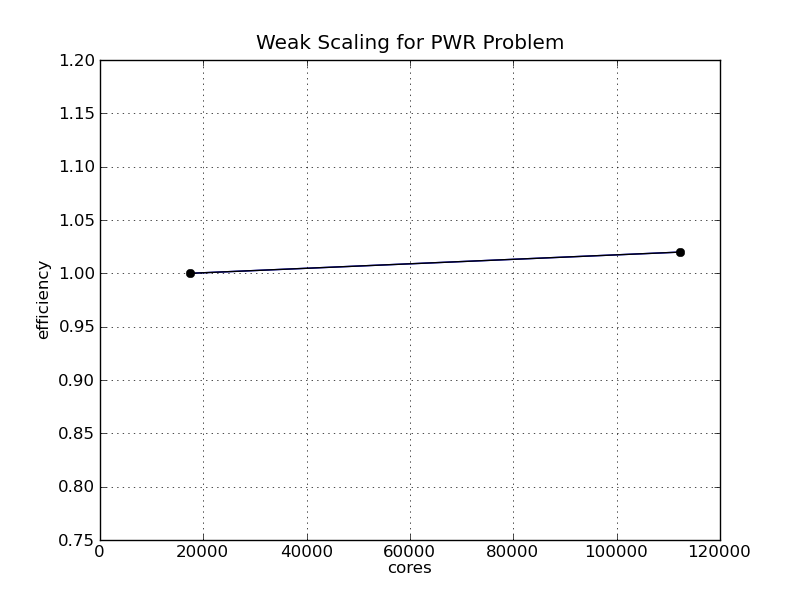
\includegraphics [width=.8\textwidth, height=0.48\textheight ] {PWRmyWeakScaling}
  \end{center}
  \caption{Weak Scaling Study for the Full PWR Calculation}
  \label{fig:PWRweakScaling}
\end{figure}

%-----------------------------------------------------
\subsection{Implications}
The tests just discussed showed that the MG Krylov solver provides a time benefit both from the parallelization in energy that is enabled by this method and from using a Krylov solver for the equivalent of the outer iterations. The author was unable to find another deterministic transport code that decomposes the upscatter calculation in energy nor one that only uses one iteration level for the upscattering block. This decomposition is a new contribution to the field and helps alleviate the scaling limitations discussed earlier.   

There are a few reasons this has not been pursued before, primarily based on computer architecture and existing code capability. Memory has only become large enough to accommodate the necessary Krylov subspaces recently. Only in the last several years have there been computers with enough processing capability to allow for scaling to hundreds of thousands of cores, motivating energy decomposition. In addition, the inner-outer paradigm is at the core of most transport codes and in many cases it would take substantial effort to modify that structure. 

Note that an explicit block Jacobi method, which converges more slowly than GS by a factor of two, could have been used previously to decouple energy groups because it is explicit in energy and does not have the large memory footprint associated with Krylov methods. However, there was no need to scale to so many cores and so there was no motivation for this development. Now that the scaling need exists, there is sufficient memory for Krylov methods. Krylov methods are the clear choice because they often converge faster than GS \cite{LeVeque2007}. 

Overall, the strong scaling studies showed that the block Krylov solver works and provides reasonably good strong scaling in both energy and space, at least out to 100,000 cores. Each test problem illustrated that the block Krylov method solves fixed source problems with upscattering more quickly than the Gauss Seidel method. The weak scaling study showed that when compared to GS, the MG Krylov method has very good weak scaling properties. This new method decisively accomplishes the goal of accelerating transport calculations by using new computers fully.

